\chapter{Results and Discussion}
\label{chapter:results}
Since the data doesn't have labels indicating which entries are anormalies, numerical evaluation is not possible. To examine how the methods perform, user interpretation of the data is the only standard. To help strength intuitive understanding, a visualization method t-SNE\cite{maaten2008visualizing} was applied. This method only requires a distance metric between pairs of data entries. Then it projects the entries into a 2D space showing potential structures underlying the data. t-SNE typically places ``important'' points in the center of the drawing. The concept of ``importance'' can be understand as a special kind of density. Intuitively, points lying in dense area are less likely to be outliers.

Section~\ref{sec:clustering} and ~\ref{sec:generative} describes results obtained using clustering method and generative method respectively. Then, section~\ref{sec:discuss} compares these two methods.
\section{Clustering Method Results}
\label{sec:clustering}
The first step of applying DBSCAN is to choose parameters. As stated in section~\ref{subsec:DBSCANalgorithm}, DBSCAN is relatively robust with $k > 4$, where $k$ stands for the $k$th nearest neighbor. In this experiment, $k$ was set to 7. The distance of the $7$th nearest neghbor of all points is draw in Fig~\ref{fig:paramDBSCAN}. The figure shows that the distance begins to increase dramatically beyond 0.5. Thus, in the experiment, $Eps$ was finally set to 0.5, with $MinPts = 7$. The clustering result is shown in Table~\ref{tab:ClusterResult} and visualized in Fig~\ref{fig:ClusterResult}.
\begin{figure}[!ht]
	\begin{center}
		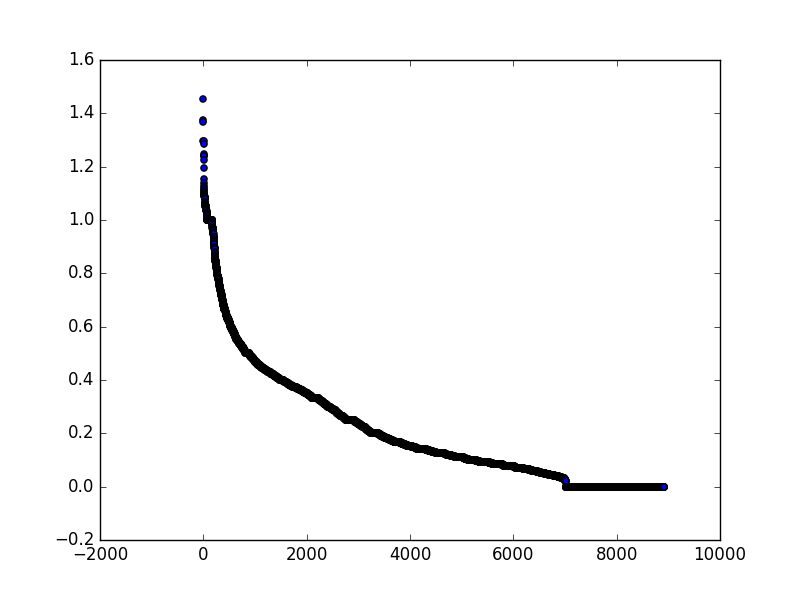
\includegraphics[width=\textwidth]{images/paramDBSCAN}
		\caption{7th nearest neighbor distance for selecting $Eps$ of DBSCAN}
		\label{fig:paramDBSCAN}
	\end{center}
\end{figure}

\begin{table}[!ht]
	\begin{center}
		\begin{tabular}{|c|c|c|c|c|c|c|c|c|c|c|c|c|}
			\hline
			Cluster No. &    0 & 1  & 2    & 3   & 4   & 5   & 6  & 7   & 8  & 9  & 10 & 11	\\ \hline
			Num Points  &  352 & 10 & 7547 & 134 & 215 & 283 & 64 & 104 & 44 & 47 & 21 & 94 \\
			\hline

		\end{tabular}
	\end{center}
	\caption{Mean, variance, and dispersion of data generated from largest department.}
	\label{tab:ClusterResult}
\end{table}

\begin{figure}[!ht]
	\begin{center}
		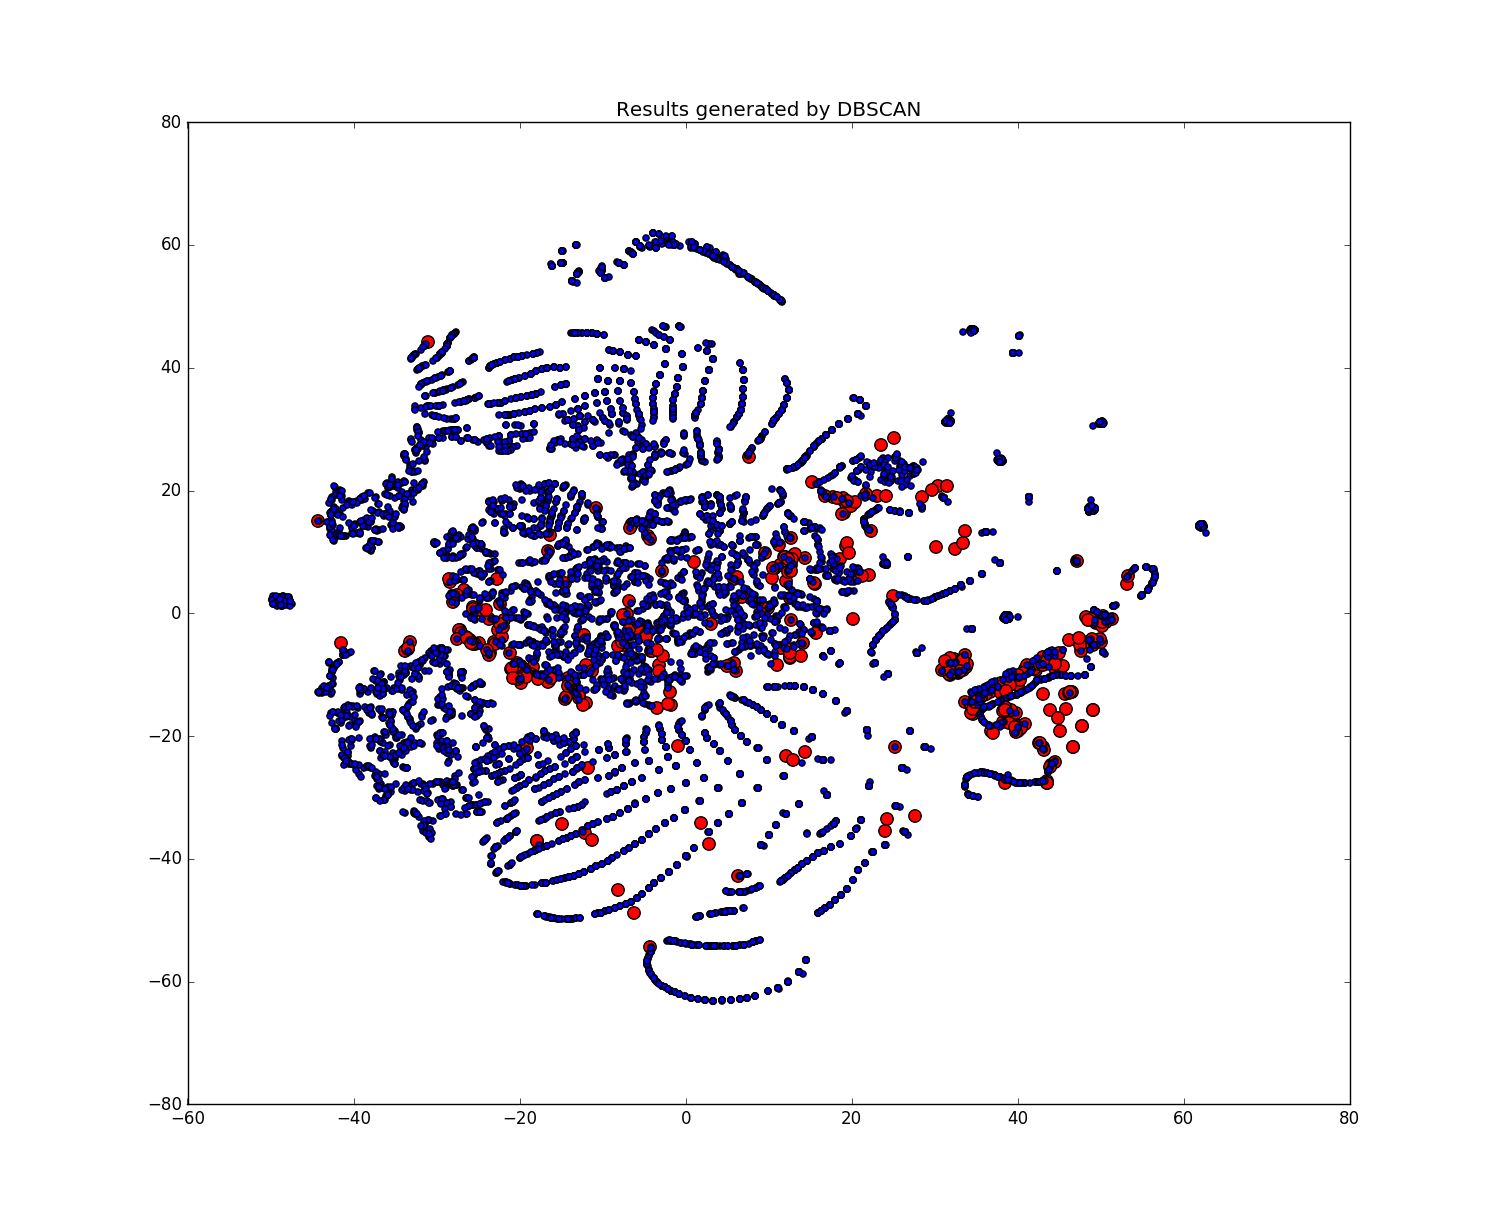
\includegraphics[width=\textwidth]{images/ClusterResult2}
		\caption{Results generated by DBSCAN, visualized using t-SNE}
		\label{fig:ClusterResult}
	\end{center}
\end{figure}

As shown in the table, 12 clusters are generated by DBSCAN. Among the 12 clusters, cluster 0 is labeled as noise/anomalies which consists of 352 visits. Cluster No.~2 is the largest cluster which consists of 7547 visits. This cluster is believed to consists of the most typical visits. For the rest small clusters, they can be considered as representing some non-typical but normal visits. One potential reason of generating such subclusters is that, there are many different resources/machines for diagnosing. Data in these subclusters are generated from these less frequently used resources/machines.

In Fig~\ref{fig:ClusterResult}, cluster 0 is plotted using red while the rest clusters are all painted in blue. As the figure shows, many red points located on the border of the figure, which indicates they come from a sparser area in their original space and have less importance. This corresponds the intuition interpretation.

To further verify the suspection, 10 samples from each cluster are listed in Table~\ref{tab:samplesFromCluster}. Visits in Cluster 0 seem very uncommon. Some visits just ended without neither closed by the doctor nor cancelled by the patient. Cluster 1 consists of similiar visits. Cluster 2 seems to have many reasonable visits. Visits from this cluster typically consists of four events and each event has duration no longer than 30 minutes. Thus, this cluster can be interpreted as the collection of normal visits as assumed. The rest clusters also exhibit some intuitive patterns. Some small clusters can be also considered as anomalies in addition to cluster 0, for example, cluster 10. The reason there are many clusters is that the distance between border points in two clusters are too large so that the two clusters did not merge. 

\section{Generative Method Results}
\label{sec:generative}
Compared to DBSCAN, Markov Chain method is easier to implment. However, some special rules need to be set before running the method. The first rule is how to handle the -1 appeared in each event, which means the visit terminates. Since negative binomial only defines probability for non-negative inputs, the probability of duration equals -1 is undefined. In the experiment, we set this probability to be the frequency of being -1 happened in this event. So the summation of the probability of all possible values is slightly larger than 1. But this does not incur large effect.

Another caveat is the numerical issues while computing likelihood. Since the likelihood of a probability will typically be so small that precision problem may occur. To avoid this, the log-likelihood is computed instead. Visits having longer sequence of events tend to have smaller likelihood, but this does not mean the visit is less likely to happen. Considering this problem, the final log-likelihood is normalized by dividing the length of the sequence. The log-likelihood of visits sorted in decreasing order is shown in Fig~\ref{fig:likelihood}. As shown by the figure, most visits have a log-likelihood larger than -10, the rest few visits with log-likelihood much smaller than -10 are very like to be anomalies. After selecting a threshould to be -10, the detection result is shown in Fig~\ref{fig:MarkovResult}. Anomalies are painted in red. Again, these suspected anomalies locates on border areas in the figure.

Similiarly, for every 1000 visits, 5 samples are selected with their log-likelihood listed in Table~\ref{tab:samplesFromGenerative} for further exploration. As listed in the table, visits in the first several blocks are very similiar and seem to be very normal. It was only from the last but one block, visits start to behave in different ways. And in the last block, which consists of visits have very large negative values of log-likelihood, these visits are very bizzare and are exactly the anomalies we tried to find.


\begin{figure}
	\begin{center}
		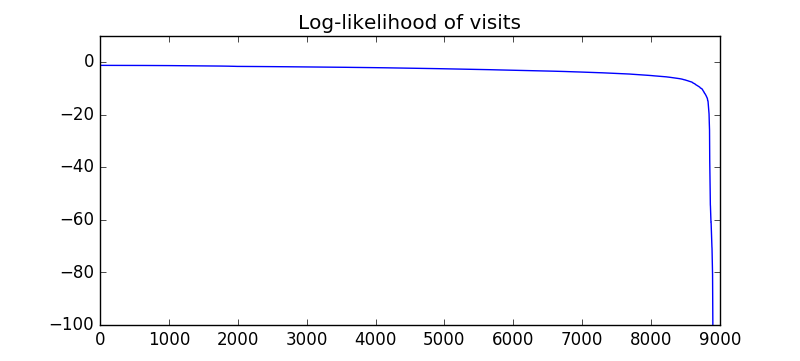
\includegraphics[width=\textwidth]{images/likelihood}
		\caption{Log-likelihood of all visits sorted in decreasing order.}
		\label{fig:likelihood}
	\end{center}
\end{figure}

\begin{figure}
	\begin{center}
		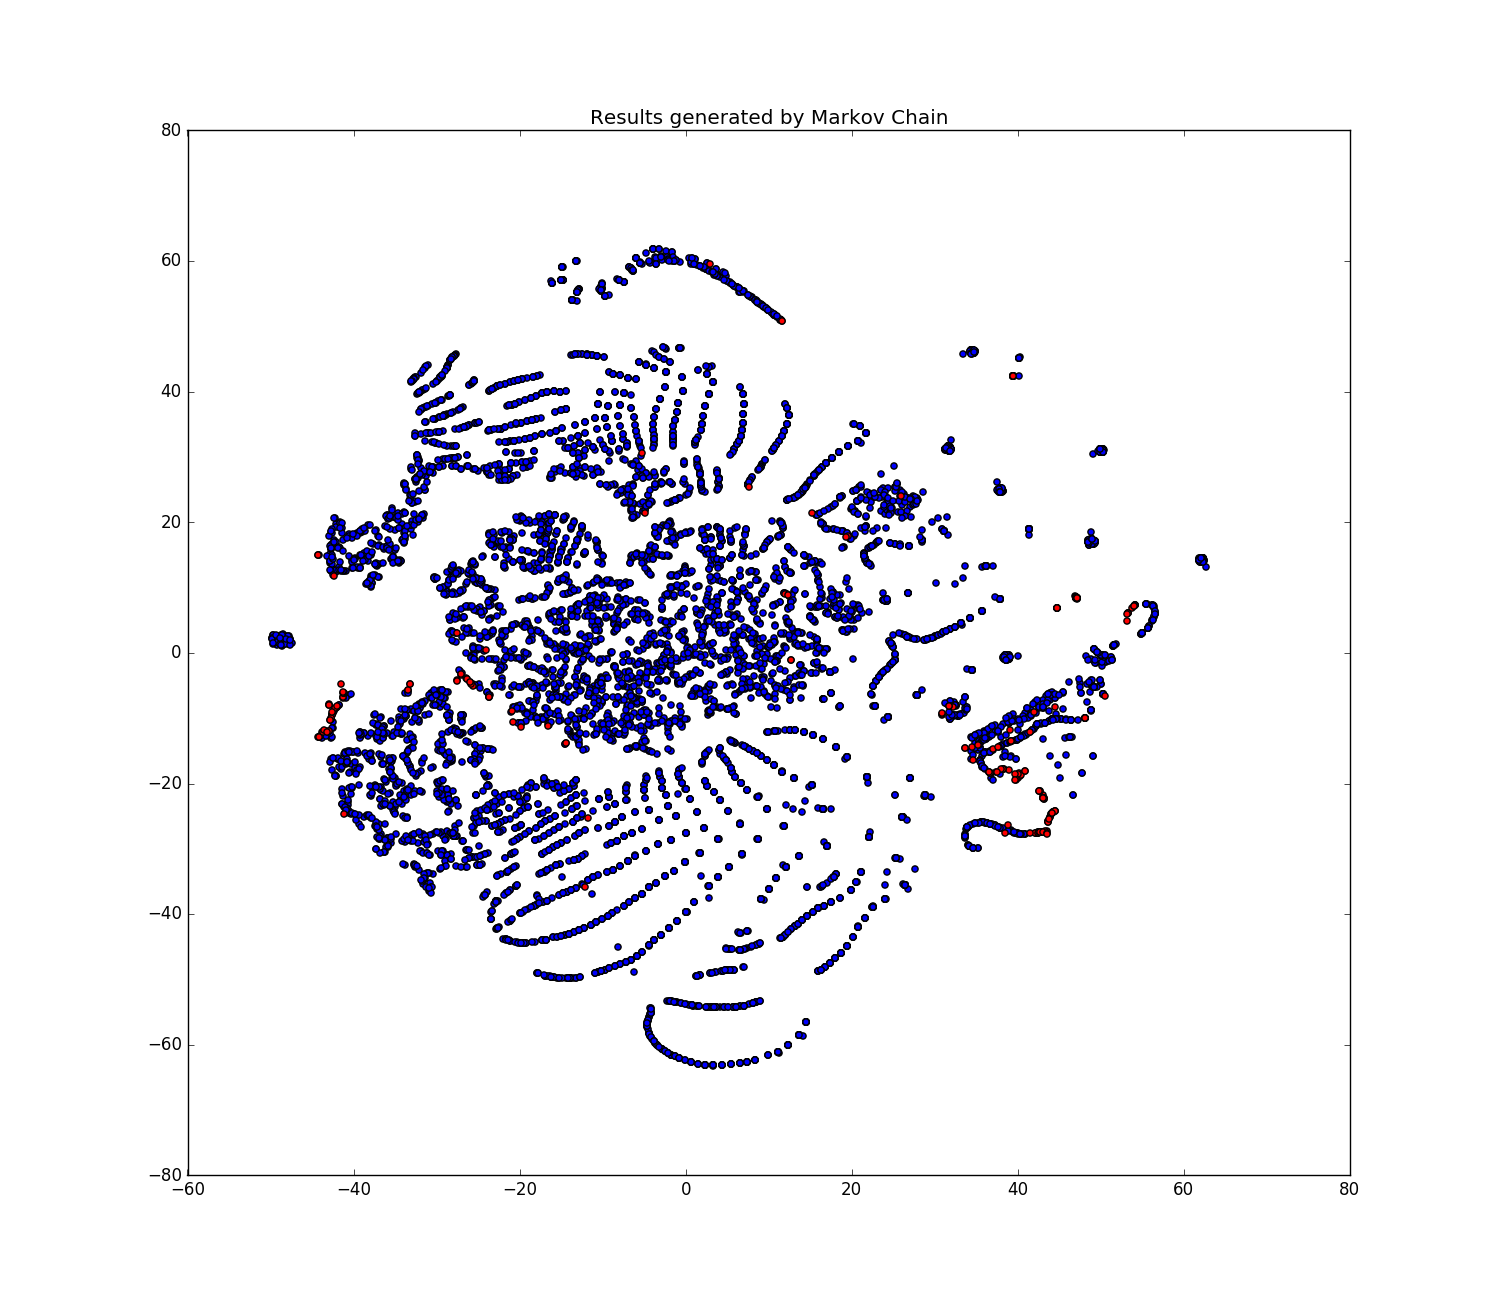
\includegraphics[width=\textwidth]{images/MarkovResult}
		\caption{Results generated by first-order Markov Chain using negative binomial distribution as emission function, visualized using t-SNE. Anomalies are painted in red.}
		\label{fig:MarkovResult}
	\end{center}
\end{figure}

\section{Discussion}
\label{sec:discuss}
Above result suggests both DBSCAN and Markov Chain can spot out anomalies. However, compared to DBSCAN, we think Markov Chain is a better method for several reasons. 

Firstly, clusters formed by DBSCAN are sligtly contaminated. For example, the 4th visit in cluster 7 seems very abnormal and should appear in other clusters. Other clusters also have entries does not resemble other visits in this log. A reason for such behavior is the hard assignment to clusters in DBSCAN. In Markov Chain, however, each visit is assigned by a score which indicates how ``normally'' this visit is. This ``soft-assignment'' is a better description of the entries. Besides, the user has to interpret the meaning of each cluster by themselves, which is typically unexpected by the user.

Secondly, Markov Chain has better time and space complexity for detecting future anomalies. When determine if a new visit log is anomaly, DBSCAN will compare this new visit to all past visits and then assign this new visit to the cluster fitting it best. Thus, DBSCAN requires to maintain all past visits, and new detection takes $O(n)$ time. This requirement will gradually becomes impractical. In contrast, Markov Chain only needs to maintain the computed parameters of transition matrix and emission functions. Computing the log-likelihood takes $O(1)$ time for each new visit log. Thus, speaking from this aspect, Markov Chain is a much better method than DBSCAN.